\documentclass[a4paper]{article} % you can use the same options as for article class

%%%%%%%%%%%%%%%%%%%%%%%%%%%%%%%%%%%%%% Meta Information %%%%%%%%%%%%%%%%%%%%%%%%%%%%%%%%%%%%%%

\def\muni{Masaryk University}
\def\uvt{Institute of Computer Science}
\def\street{Botanick\'{a} 68a}
\def\psc{602\,00 Brno}

\def\projectname{AIDA Framework}

\def\reportauthor{Martin Hus\'{a}k, Jaroslav Ka\v{s}ar, Milan \v{Z}iaran}
\def\reporttitle{User Manual \& Documentation}

%%%%%%%%%%%%%%%%%%%%%%%%%%%%%%%%%%%%%% Included Packages %%%%%%%%%%%%%%%%%%%%%%%%%%%%%%%%%%%%%%

\usepackage[paper=a4paper,top=2.5cm,bottom=2.5cm,left=2.5cm,right=2.5cm,bottom=2.5cm,foot=1cm]{geometry}
\usepackage{cmap}       % cut and past support for iso-8859-2 characters
\usepackage[utf8]{inputenc}
\usepackage[default,osfigures,scale=0.5]{opensans}
\usepackage[T1]{fontenc}
\usepackage[hyphens]{url}
\usepackage{hyperref}
\usepackage[usenames, dvipsnames]{xcolor}
% \usepackage{lastpage}
\usepackage{indentfirst}
\usepackage{graphicx}
% \usepackage{booktabs}
% \usepackage{multirow}
\DeclareGraphicsExtensions{.pdf, .ps, .eps, .png}

%%%%%%%%%%%%%%%%%%%%%%%%%%%%%%%%%%%%%% Colors %%%%%%%%%%%%%%%%%%%%%%%%%%%%%%%%%%%%%%

\definecolor{projectcolor}{RGB}{93,118,168}
\definecolor{uvtcolor}{RGB}{188,4,78}
\definecolor{textcolor}{RGB}{90,90,90}
\definecolor{notecolor}{RGB}{150, 150, 150}
\definecolor{emphcolor}{RGB}{93,118,168}

%%%%%%%%%%%%%%%%%%%%%%%%%%%%%%%%%%%%%% Settings for pdf output %%%%%%%%%%%%%%%%%%%%%%%%%%%%%%%%%%%%%%

\hypersetup{%
pdftitle   = {\reporttitle},
pdfauthor  = {\reportauthor},
pdfsubject = {\projectname},
pdfkeywords= {},
%
unicode=true,                % czech in bookmarks
bookmarks=true,              % turn on creation of bookmarks
bookmarksopen=false,         % expand subsections in bookmark tab
bookmarksnumbered = true,    % chapter numbers in bookmarks
bookmarksopenlevel = 5,
%
pdfpagemode=UseOutlines,     % UseThumbs, UseOutlines (turn on bookmarks), FullScreen, None
pdfpagelayout=SinglePage,    % SinglePage, OneColumn, TwoColumnLeft, TwoColumnRight
pdfstartview=FitV,           % Fit, FitB, FitH, FitV
%
backref = false,
linkcolor = textcolor,
citecolor = textcolor,
urlcolor = textcolor,
colorlinks = true,           % on/off link boxes
hyperindex=true,
plainpages=false,            % fix duplicated pages when roman/arabic numbering is used
%
}

%%%%%%%%%%%%%%%%%%%%%%%%%%%%%%%%%%%%%% Document formating %%%%%%%%%%%%%%%%%%%%%%%%%%%%%%%%%%%%%%

\renewcommand{\sfdefault}{opensans}
\renewcommand{\familydefault}{\sfdefault}
\renewcommand{\normalsize}{\fontsize{12}{15}\selectfont\color{textcolor}}

\tolerance 9999 % big white space tolerance for better typesetting and text hyphenation

\def\verbatim@font{\color{textcolor}} % color of verbatim text

\makeatletter       % section title formating
\renewcommand\section{\@startsection {section}{1}{\z@}%
                   {-3.5ex \@plus -1ex \@minus -.2ex}%
                   {2.3ex \@plus.2ex}%
                   {\normalfont\sffamily\Large\bfseries\color{projectcolor}}}
\renewcommand\subsection{\@startsection{subsection}{2}{\z@}%
                   {-3.25ex\@plus -1ex \@minus -.2ex}%
                   {1.5ex \@plus .2ex}%
                   {\normalfont\sffamily\large\bfseries\color{projectcolor}}}
\renewcommand\subsubsection{\@startsection{subsubsection}{3}{\z@}%
                   {-3.25ex\@plus -1ex \@minus -.2ex}%
                   {1.5ex \@plus .2ex}%
                   {\normalfont\normalsize\sffamily\bfseries\color{projectcolor}}}
\makeatother

\newenvironment{itemize*}%
{\begin{itemize}%
    \setlength{\itemsep}{0pt}%
    \setlength{\parskip}{0pt}%
}{\end{itemize}}

\usepackage[pages=some,scale=1,angle=0,opacity=1]{background}
\newcommand\BackImage[2][scale=1]{%
\BgThispage
\backgroundsetup{
  contents={\includegraphics[#1]{#2}}
  }
}
\usepackage[absolute,overlay]{textpos}

% fancy verbatim and listings
\usepackage{fancyvrb}
\usepackage{listings}
\definecolor{listingbg}{RGB}{242,242,242}
\lstset{
	basicstyle=\footnotesize\ttfamily,
	captionpos=b,
	backgroundcolor=\color{listingbg},
	framesep=4pt,
	frame=single,
	breaklines=true,
	rulecolor=\color{listingbg},
	aboveskip=10pt
}

\begin{document}

% title page
{
\BackImage[width=1.4\textwidth]{fig/titlepage_bg}
\pdfbookmark[1]{Title page}{pdf_first_page}

\vspace*{5cm}

\color{white}
  \begin{center}
  \vspace{2cm} {\Huge \projectname}

  \vspace{1cm} {\huge\bfseries\MakeUppercase{\reporttitle}}
  \end{center}

  \begin{textblock}{3}(1,10)
      \hyphenpenalty=10000 % prevent names from hyphenating
         \begin{tabular}{rl }
            Authors & \reportauthor \\
             & \\
            Contact address & \muni \\
             & \uvt \\
             & \street \\
             & \psc \\
          \end{tabular}
      \hyphenpenalty=0
  \end{textblock}
  \cleardoublepage
}

\normalfont

% content page

\pdfbookmark[1]{Content}{pdf_contents}

\setcounter{tocdepth}{3}

\tableofcontents

\vspace*{\fill}

\normalfont

\pdfbookmark[1]{Acknowledgement}{Acknowledgement}
\section*{Acknowledgment}

The authors of the AIDA framework are Martin Hus\'{a}k, Jaroslav Ka\v{s}ar, and Milan \v{Z}iaran. The authors would like to thank Michal Pav\'{u}k, V\'{i}t Rus\v{n}\'{a}k, and Jakub Kolman for the dashboard, and Petr Velan and Samuel \v{S}u\v{l}an for testing the framework.

% AIDA Framework integrates SPMF library\footnote{\url{http://www.philippe-fournier-viger.com/spmf/}} distributed under GPL v3 license.

There is a design paper describing the AIDA framework, see:
\begin{lstlisting}[]
Martin Husák and Jaroslav Kašpar. 2019. AIDA Framework: Real-Time Correlation and Prediction of Intrusion Detection Alerts. In Proceedings of the 14th International Conference on Availability, Reliability and Security (ARES '19). ACM, New York, NY, USA, Article 81, 8 pages. DOI: https://doi.org/10.1145/3339252.3340513
\end{lstlisting}

To cite the paper, we recommend using the following bibtex entry:
\begin{lstlisting}[]
@inproceedings{AIDAframework,
 author = {Hus\'{a}k, Martin and Ka\v{s}par, Jaroslav},
 title = {AIDA Framework: Real-Time Correlation and Prediction of Intrusion Detection Alerts},
 booktitle = {Proceedings of the 14th International Conference on Availability, Reliability and Security},
 series = {ARES '19},
 year = {2019},
 isbn = {978-1-4503-7164-3},
 location = {Canterbury, CA, United Kingdom},
 pages = {81:1--81:8},
 doi = {10.1145/3339252.3340513},
 publisher = {ACM},
 address = {New York, NY, USA},
 keywords = {alert correlation, data mining, information sharing, intrusion detection, prediction}
}
\end{lstlisting}

The development of the framework and related research were supported by the Security Research Programme of the Czech Republic 2015 - 2020 (BV III / 1 VS) granted by the Ministry of the Interior of the Czech Republic under No. VI20162019029 The Sharing and analysis of security events in the Czech Republic. 
Further research was supported by ERDF ``CyberSecurity, CyberCrime and Critical Information Infrastructures Center of Excellence'' (No.CZ.02.1.01/0.0/0.0/16\_019/0000822).

\cleardoublepage

\section{Introduction}

AIDA is an analytical framework for processing intrusion detection alerts with a focus on alert correlation and predictive analytics. The framework contains components that filter, aggregate, and correlate the alerts, and predict future security events using the predictive rules distilled from historical records. The components are based on stream processing and use selected features of data mining (namely sequential rule mining) and complex event processing. The framework was designed to be deployed as an analytical component of an alert processing platform. Alternatively, it can be deployed locally for experimentations over datasets.

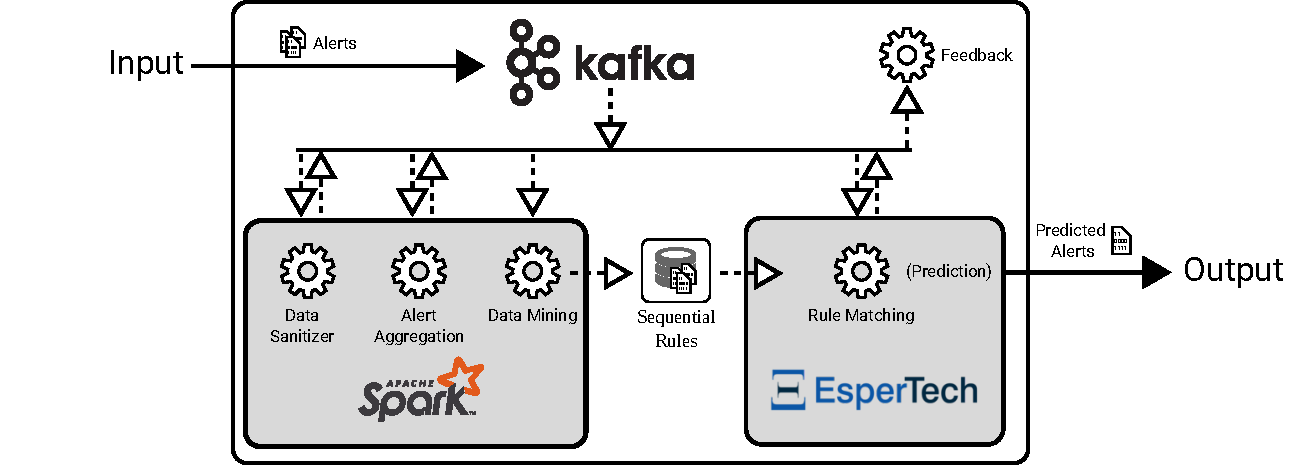
\includegraphics[width=\textwidth]{fig/aida_schema}

IDEA\footnote{\url{https://idea.cesnet.cz/}}

\begin{lstlisting}[]
OrganizationA.Honeypot1_Recon.Scanning_22,
OrganizationB.IDS1_Attempt.Login_22
==>
OrganizationA.IDS1_Attempt.Login_22
#SUPP: 0.0011 #CONF: 0.6111
\end{lstlisting}

\begin{lstlisting}[]
{
  "Format": "IDEA0",
  "ID":"f62537c2-77b8-49c7-a0a2-24c4b81b20f8",
  "CorrelID": [ % IDs of preceding alerts
        "3688762d-2efa-44a8-9ea5-34a57b3ae0c7",
        "ae6d9ac6-6389-407f-9d7e-58b9692c6eaa"
      ],
  "DetectTime": "2019-03-16T12:17:21.609+00:00",
  "Category": ["Attempt.Login"],
  "Confidence": "0.6111",
  "Description": "The source IP address follows a known pattern that is expected to continue with the event described in this message.",
  "Note": "OrganizationA.Honeypot1_Recon.Scanning_22, OrganizationB.IDS1_Attempt.Login_22 ==> OrganizationA.IDS1_Attempt.Login_22",
  "Source": [{"IP4": ["10.11.12.13"]}],
  "Target": [{"Port":[22]}],
  "Node": [
    { % Node referencing the AIDA Framework
      "Name": "OrganizationX.AIDA",
      "SW": "AIDA",
      "Type": ["Correlation", "Statistical"]
    },
    { % Node derived from the rule
      "Name": "OrganizationA.IDS1"
    }
  ]
}
\end{lstlisting}

\cleardoublepage

\section{Quick Start}

For a quick start, go to the provision directory and run Vagrant:

\begin{lstlisting}[]
cd provision
\end{lstlisting}

\begin{lstlisting}[]
vagrant up
\end{lstlisting}

AIDA framework will start in few minutes. Then, send your data to the framework using the following command (you need to have netcat installed):

\begin{lstlisting}[]
nc localhost 4164 < path_to_file_with_your_data
\end{lstlisting}

If you do not have your own data, we recommend trying AIDA framework out with our dataset\footnote{\url{http://dx.doi.org/10.17632/p6tym3fghz.1}}. Download and unzip the main file in the datase (dataset.idea.zip) and use it in the command above.

TODO run data mining

TODO update rules

TODO check outputs

\cleardoublepage

\section{Installation Instructions}

deployment

\subsection{Prerequisities}

\subsection{Installation}

h1. Instalace iABU na testbedu

h2. Java

Java je nainštalovaná nasledovným spôsobom:
* najnovšia verzia (jdk-8u92) stiahnutá z webu Oracle
* pomocou java-package zostavený balík .deb
* .deb následne nainštalovaný do systému

OpenJDK 8 nainstalováno z backport balíku
* přidaný zdroj "deb http://ftp.cz.debian.org/debian jessie-backports main" v /etc/apt/sources.list


h2. Maven

Standardní instalace Apache Maven 3.0.5
Maven home: /usr/share/maven

h2. Python

Téměř všechny nástroje používají python verze 3 (krom Warden klienta).
Nainstalované balíčky (pro python3):
\begin{lstlisting}[]
python-daemon==2.1.2
kafka-python==1.4.1
ujson==1.35
python-dateutil==2.6.1
neo4j-driver==1.4.0
\end{lstlisting}

h2. Uživatelé

Vytvoření uživatelé
* spark (běží pod ním spark a všechny spark aplikace)
** groups=sudo
* iabu (beží pod ním všechno ostatní)

h2. Warden client

h2. Mentat inspector

h2. Kafka

Kafka je nainstalovaná ve složce @/opt/kafka/@

\begin{lstlisting}[]
$ mkdir /opt/kafka
$ cd /opt/kafka
$ wget http://apache.miloslavbrada.cz/kafka/0.10.0.1/kafka_2.11-0.10.0.1.tgz -O kafka.tgz
$ tar -xzf kafka.tgz --strip-components=1
$ rm kafka.tgz
$ sudo chown -R iabu:iabu ./
\end{lstlisting}

Zmenit nastaveni 'log.dirs=/var/tmp/kafka-logs' v /opt/kafka/config/server.properties - nevím jeslti to pomůže, ale padla nám kafka na "ERROR Error while appending records to input-0 in dir /tmp/kafka-logs (kafka.server.LogDirFailureChannel) java.io.IOException: No space left on device".

h2. Kafka filer

Čte události z file systému a posílá je do kafka topicu. 
V repozitáři je i kafka\_warden\_filer.py, což je modifikovaný warden client, který neukládá idea zprávy na file systém, ale do kafka topicu. (Momentálně nepoužívaný)

Skript z repozitáře @/kafka-filer/kafka\_filer.py@ vložit do @/opt/kafka\_filer.py@.

\begin{lstlisting}[]
$ sudo chown iabu:iabu /opt/kafka_filer.py
$ sudo chmod u=rwx,g=rx,o=g /opt/kafka_filer.py
\end{lstlisting}

h2. Spark

Spark je nainstalován ve složce @/opt/spark/@

\begin{lstlisting}[]
$ mkdir /opt/spark
$ cd /opt/spark
$ wget http://apache.miloslavbrada.cz/spark/spark-2.2.0/spark-2.2.0-bin-hadoop2.7.tgz -O spark.tgz
$ tar -xzf spark.tgz --strip-components=1
$ rm spark.tgz
$ sudo chown -R spark:spark ./
\end{lstlisting}

V homu uživatele Spark je potřeba připravit prostředí pro spouštění kafky a kafka aplikací.
* je potřeba vytvořit adresář @/home/spark/applications@
* vložit do něj skripty pro spuštění/vypnutí spark clusteru a spouštění spark aplikací
** z repozitáře @/common/spark/scripts@
* Stáhnout @spark-streaming-kafka-assembly.jar@ do daného adresáře.
** \begin{lstlisting}[]
$ cd /home/spark/applications
$ wget -O spark-streaming-kafka-assembly.jar http://search.maven.org/remotecontent?filepath=org/apache/spark/spark-streaming-kafka-0-8-assembly_2.11/2.1.0/spark-streaming-kafka-0-8-assembly_2.11-2.1.0.jar
\end{lstlisting}

h2. Spark aplikace

Spark aplikace jsou umístěné v repozitáři a spouští se pomocí skriptu @/home/spark/applications/run-application.sh@.
Pro jednoduchou a snadnou aktualizaci aplikací je celý repozitář naklonován ve složce @/home/spark/applications/sabu@ odkud se aplikace spouštějí.

\begin{lstlisting}[]
$ git clone git@homeproj.cesnet.cz:sabu /home/spark/applications/sabu
\end{lstlisting}

h2. Neo4j

* nainstalované z balíčku (přidaný zdroj /etc/apt/sources.list.d/neo4j.list)
* web interface běží na portu 7474 (http://sabu-testbed.cesnet.cz:7474)
** jméno neo4j, heslo sabu.matrix
* viz konfigurace v /etc/neo4j/neo4j.conf

h2. iptables

* V současné době je omezen přístup na porty 8080-8090 a 4040-4060 (Spark web GUI), 7474 (Neo4j), 27017 (Mongo), 2181 a 9092 (Kafka) pouze se sítě MU:
\begin{lstlisting}[]
$ cat /etc/network/run/iptables.conf
*filter
# Set drop as default
:INPUT DROP
# Spark publicly accessed only from the network 147.251.0.0/16
-A INPUT -i eth0 -p tcp -m multiport --dports 7474,8080:8090,4040:4060,27017,2181,9092 ! -s 147.251.0.0/16 -j DROP
# Allow everything
-A INPUT -p all -j ACCEPT
COMMIT
\end{lstlisting}

h1. --------------------------
Staré - smazat

h2. Warden (Mentat)

Warden je nainštalovaný pomocou git repozitára:
\begin{lstlisting}[]/opt/warden3/\end{lstlisting}
Súbory warden_filer_reciever (sender je neaktívny):
\begin{lstlisting}[]/etc/init.d\end{lstlisting}
Konfiguračný súbor pre filer:
\begin{lstlisting}[]/etc/warden_filer.cfg\end{lstlisting}
Momentálne prebieha sťahovanie udalostí z Wardenu do zložky napojenej na Mentat:
\begin{lstlisting}[]/var/mentat/spool/_enricher/incoming/\end{lstlisting}

h2. Warden (Spark)

Na testbede je momentálne zaregistrovaný aj druhý klient (receiver) pre potreby čističky.

Jednotlivé filery vrátane konfiguračných súborov sú v zložke:
\begin{lstlisting}[]/opt/warden3-spark/contrib_3.0-beta2/warden_filer/\end{lstlisting}

Popis viacerých verzií je v súbore GUIDE

h3. HDFS

* Dáta spracovávané Sparkom sa ukladajú do:
\begin{lstlisting}[]/opt/warden3-spark/contrib_3.0-beta2/warden_filer/warden_receiver/incoming\end{lstlisting}

* Filer je upravený pre mazanie správ starších > 60/300s (nastavuje sa v skripte):
\begin{lstlisting}[]./warden_filer.py receiver -d\end{lstlisting}


h3. Kafka

* Pri nastavení oboch parametrov (topic, zookeper) ukladá do Kafky, inak súbory:
\begin{lstlisting}[]./warden_filer.py receiver -d -k <topic_name> -z <ip:port>\end{lstlisting}

\subsection{Setup}

h1. Postup zprovoznění iABU

* nasazeno a provozováno na sabu-testbed.cesnet.cz
* v systému je připraven uživatel iabu, pod kterým by všechny nástroje měly běžet
* doporučené umístění souborů:
** nástroje/binárky - /opt/
** konfigurace - /etc/iabu/
** data - /var/iabu/
** logy - /var/log/iabu/
** pid\_files - /var/run/iabu/

h2. Tok dat v systému

\begin{lstlisting}[]
-----------------                                 -------------                                  ---------------                                 ----------------------------                           -------------------------------
| warden client | -> /var/iabu/warden_receiver -> | inspector | -> /var/iabu/mentat_inspector -> | kafka filer | -> kafka topic: warden-input -> | Spark app: Deduplication | -> kafka topic: marked -> | Spark apps: Graph-db, Miner | -> neo4j database, /var/iabu/analyzer/miner
-----------------                                 -------------                                  ---------------                                 ----------------------------                           -------------------------------
\end{lstlisting}

h2. Warden klient

* Spuštění
\begin{lstlisting}[]
$ sudo -u iabu python /usr/local/bin/warden_filer.py receiver -c /etc/iabu/warden_filer.cfg --pid_file /var/run/iabu/warden_receiver.pid -d
\end{lstlisting}

* Výstup
\begin{lstlisting}[]
/var/iabu/warden_receiver
\end{lstlisting}

h2. Inspector

* Spuštění
\begin{lstlisting}[]
$ sudo -u iabu python3 /usr/local/bin/mentat-inspector.py --config-file /etc/iabu/inspector.cfg --pid-file /var/run/iabu/inspector.pid --log-file /var/log/iabu/inspector.log
\end{lstlisting}

* Vstup
\begin{lstlisting}[]/var/iabu/warden_receiver
\end{lstlisting}
* Výstup
\begin{lstlisting}[]
/var/iabu/mentat_inspector
\end{lstlisting}

h2. Kafka

Nejdříve je potřeba spustit zookeeper (port 2181), který používá kafka pro ukládání konfigurace. Poté je potřeba spustit samotný kafka broker (port 9092).

* Spuštění Zookeeperu
\begin{lstlisting}[]
$ sudo -u iabu /opt/kafka/bin/zookeeper-server-start.sh -daemon /opt/kafka/config/zookeeper.properties
\end{lstlisting}

* Spuštění Kafky
\begin{lstlisting}[]
$ sudo -u iabu /opt/kafka/bin/kafka-server-start.sh -daemon /opt/kafka/config/server.properties
\end{lstlisting}

* Vypsání existujících topiců
\begin{lstlisting}[]
$ /opt/kafka/bin/kafka-topics.sh --list --zookeeper localhost:2181
\end{lstlisting}
** Pokud *warden-input* nebo *marked* neexistují, je potřeba je vytvořit
\begin{lstlisting}[]
$ /opt/kafka/bin/kafka-topics.sh --create --zookeeper localhost:2181 --replication-factor 1 --partitions 1 --topic warden-input
$ /opt/kafka/bin/kafka-topics.sh --create --zookeeper localhost:2181 --replication-factor 1 --partitions 1 --topic marked
\end{lstlisting}
** Připadné smazání topicu
\begin{lstlisting}[]
$ /opt/kafka/bin/kafka-topics.sh --delete --zookeeper localhost:2181 --topic topic-name
\end{lstlisting}

* Spuštění konzolového konzumenta a producera pro testování:
\begin{lstlisting}[]
$ /opt/kafka/bin/kafka-console-producer.sh --broker-list localhost:9092 --topic warden-input
$ /opt/kafka/bin/kafka-console-consumer.sh --bootstrap-server localhost:9092 --topic warden-input --from-beginning
\end{lstlisting}

* Zjištění aktuálního stavu čtení konkrétního konzumenta z topiců
\begin{lstlisting}[]
$ /opt/kafka/bin/kafka-consumer-groups.sh --bootstrap-server localhost:9092 --group esper-event-matcher --describe
\end{lstlisting}

* Posunutí offsetu konkrétní consumer group na posledni zprávu
\begin{lstlisting}[]
$ /opt/kafka/bin/kafka-consumer-groups.sh --bootstrap-server localhost:9092 --group [group name] --reset-offsets --to-latest --all-topics --execute
\end{lstlisting}

h2. Kafka filer

\begin{lstlisting}[]
$ sudo -u iabu python3 /opt/kafka_filer.py -d /var/iabu/mentat_inspector/incoming -t warden-input -z localhost:9092
\end{lstlisting}

* Vstup \begin{lstlisting}[]/var/iabu/mentat_inspector/incoming\end{lstlisting}
* Výstup jde do kafka topicu
** jméno: 'warden-input'
** zookeeper: localhost:9092

h2. Spark

Spark je nainstalovaný v _/opt/spark/_. Je pro něj vytvořený uživatel *spark*, který má v home adresáři skripty pro spouštění a vypínání spark clusteru. 
Dostupné webové rozhraní http://sabu-testbed.cesnet.cz:8080 .

* Spuštění
\begin{lstlisting}[]
sudo -u spark /var/home/spark/applications/start-cluster.sh
\end{lstlisting}
* Vypnutí  (pozor, jedna worker se zpravidla nevypne - je třeba zabít proces)
\begin{lstlisting}[]
sudo -u spark /var/home/spark/applications/stop-cluster.sh
\end{lstlisting}

Ukládání logů do  (potřeba promazávat)
\begin{lstlisting}[]
/opt/spark/work
\end{lstlisting}

h3. Spark applikace

Aplikace sparku se spouštějí každá ve svém vlastním screenu uživatele *spark* pomocí skriptu @/home/spark/applications/run-application.sh@.

h2. Deduplication (Spark aplikace)

\begin{lstlisting}[]
$ sudo su spark
$ script /dev/null
$ screen -r idea-dedupliacation
$ ~/applications/run-application.sh ~/applications/sabu/deduplication/spark/spark_app.py
Detache from screen by pressing ctrl + A + D
\end{lstlisting}

h2. Neo4J

Nainstalovaný z balíku jako služba. Dostupné webové rozhraní na http://sabu-testbed.cesnet.cz:7474/ .

\begin{lstlisting}[]
$ sudo service neo4j start
\end{lstlisting}

h2. Graph-db (Spark aplikace)

Aplikace plní Neo4j databázi událostmi z topicu *marked*.

\begin{lstlisting}[]
$ sudo su spark
$ script /dev/null
$ screen -r graph-db
$ ~/applications/run-application.sh ~/applications/sabu/analyzer/graph-db/spark/spark_app.py
Detache from screen by pressing ctrl + A + D
\end{lstlisting}

h2. Miner (Spark aplikace)

Momentálně pouze generuje SPMF databáze. Dolování vzorů a pravidel je zakomentováno.

\begin{lstlisting}[]
$ sudo su spark
$ script /dev/null
$ screen -r miner
$ ~/applications/run-application.sh ~/applications/sabu/analyzer/miner/spark/spark_app.py
Detache from screen by pressing ctrl + A + D
\end{lstlisting}

* Vstup
** kafka topic *marked*
* Výstup
\begin{lstlisting}[]
/var/iabu/analyzer/miner/
\end{lstlisting}

h2. Mazání dat

finální stav - crontab uživatele iabu (jako root: crontab -e -u iabu):
\begin{lstlisting}[]
* * * * * find /var/iabu/warden_receiver/incoming/* -mmin +1 -exec rm {} \; 2> /dev/null
* * * * * find /var/iabu/mentat_inspector/incoming/* -mmin +1 -exec rm {} \; 2> /dev/null
\end{lstlisting}

\cleardoublepage

\section{User Guide}

incl. screenshots


\includegraphics[width=0.75\textwidth]{fig/dashboard_login}

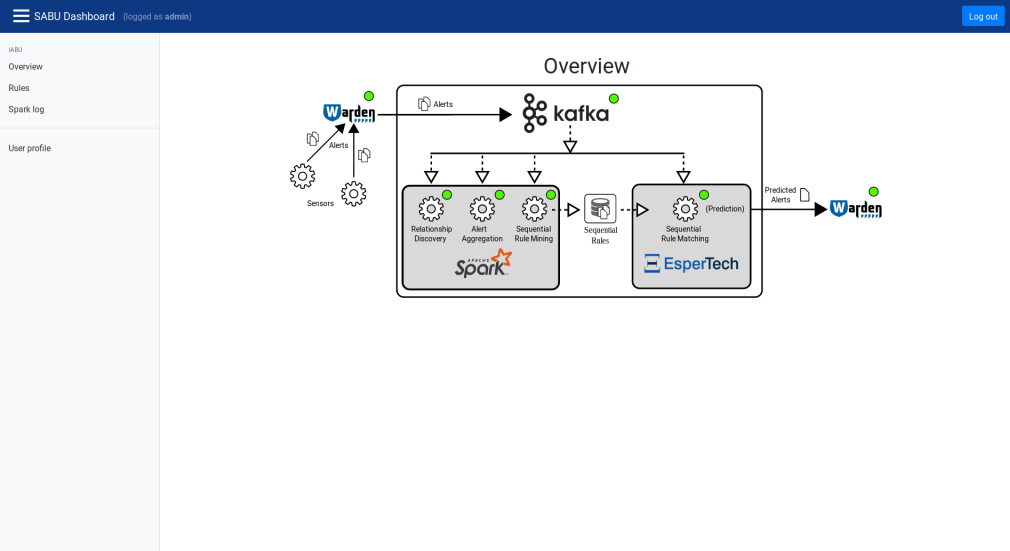
\includegraphics[width=0.75\textwidth]{fig/dashboard_overview}

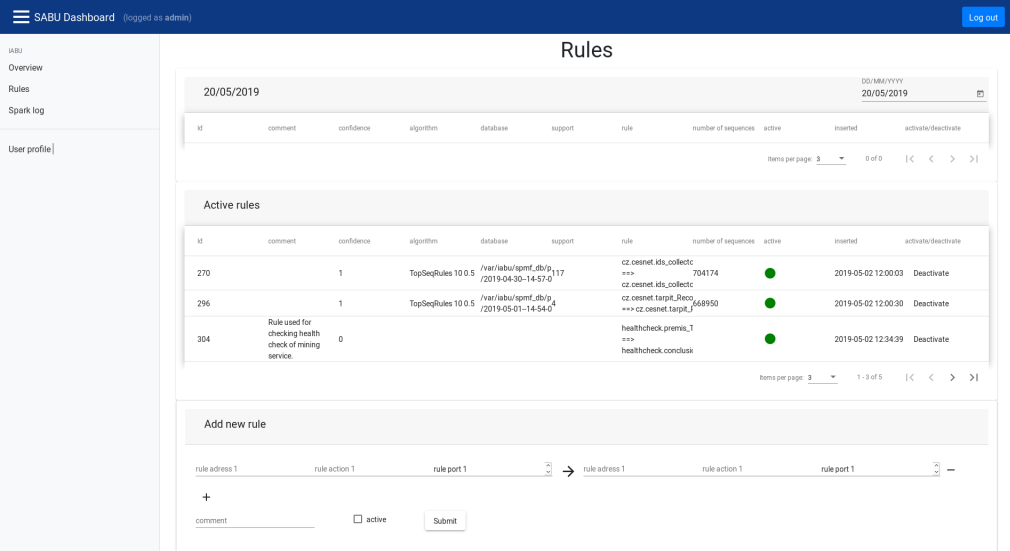
\includegraphics[width=0.75\textwidth]{fig/dashboard_rules}

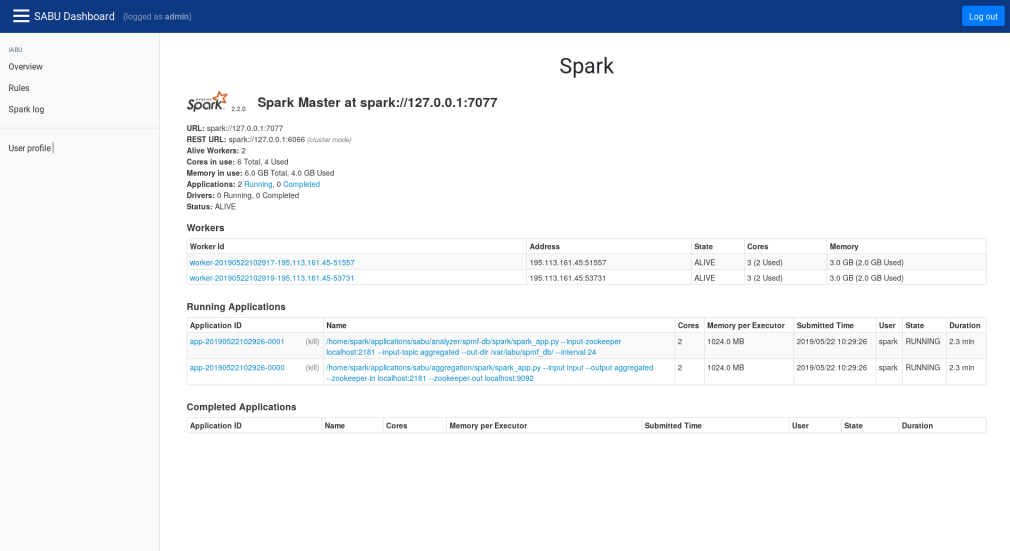
\includegraphics[width=0.75\textwidth]{fig/dashboard_spark}

\cleardoublepage

\section{Technical Documentation}

\subsection{Inputs and Outputs}

\subsection{Kafka}

\subsection{Spark}

\subsection{Sanitizer}

\subsection{Aggregation}

\subsection{Data Mining}

\subsection{Database}

\subsection{Rule Matching}

\subsection{Feedback}

\subsection{REST API}

    /componentsinfo/ - rozšířený stav komponent iABU (včetně výpisů systemd a posledních x řádků logu)

    /db/rules/YYYY-MM-DD/ - Zoznam pravidiel z daného dňa.
    /db/activerules/ - Zoznam aktívnych pravidiel.
    POST /db/activerules/id/ - Aktivuje pravidlo s daným ID.
    POST /db/inactiverules/id/ - Deaktivuje pravidlo s daným ID.
    POST /db/deleterules/id/ - Zmaže pravidlo s daným ID.
    POST /db/addrules/pravidlo/ - Vytvorí nové pravidlo.

    /enforcedatamining/ - vynutí spuštění data miningu nad současnou databází její smazání
    /reloadrulematching/ - vynutí restart Rule Matching komponenty spojený s načtením nové sady pravidel

Testovacia databáza: /var/www/restapi/sabu-test.db

\subsection{Dashboard}

\subsection{Ansbile and Vagrant}

\end{document}
